\documentclass[twocolumn, twoside,11pt,A4]{article}%
\usepackage{royce_note}
\begin{document}
\author{E. Officer}
\title{Growth of Whizzy Material}	
\twocolumn[
\begin{@twocolumnfalse}
	\maketitle\thispagestyle{fancy}
	\begin{abstract}
		This application note describes the growth of whizzy material in the Royce Insitute thin films deposition facility and presents data demonstrating the materialsd properties.
	\end{abstract}
	\rule{\textwidth}{1pt}
\end{@twocolumnfalse}
]
	
\section{Introduction}
\blindtext \cite{Mathur1997}
\blindtext \cite{AlMaMari2015}
\section{Growth}
\blindtext \cite{Hueso2007}
\blindtext \cite{Flokstra2015a}
\blindtext \cite{Shi2017}
\section{Properties}
\begin{figure}
	\centering
	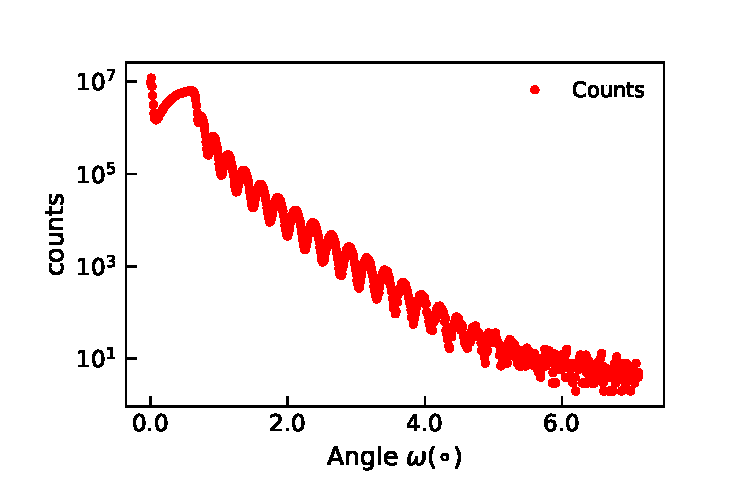
\includegraphics[width=\columnwidth]{XRR_Data}
	\label{xrr_data}
	\caption{X-ray reflectivity data of a copper thin film grown in the sputtering chamber. The fitted thickness was 30\units{nm}.}
\end{figure}
\blindtext \cite{Benitez2015}
\blindtext 
\blindtext 
\section{Further Information}
\blindtext 

\printbibliography

\end{document}